\chapter{Results}

\section{Our Contributions}

In this section we will present and reiterate the contributions we have made as a result of this project.

We have contributed with a simplified Python version of the original GFN2-xTB Fortran implementation. The implementation and validation of the dispersion term is not complete, and we are missing the anisotropic electrostatic term (AES), the anisotropic exchange correlation term (AXC), the Fermi term, and the implementation for the self-consistent charges. The most difficult part of AES and AXC is getting the S, D, and Q matrices, which we already have. Given the size of the reference implementation we are quite satisfied with this. The Python implementation should hopefully make the GFN2-xTB algorithm more approachable for our successors and give a good foundation for making the lockstep parallel GPU implementation.

We have contributed a testing framework for comparing results against the original Fortran implementation. We utilize Nix to ensure tests that are reproducible, regardless of Linux distribution and system configuration. In connection to this, we have also contributed a reproducible and easy way to build, run, and patch xtb. This also includes its dependencies, and even the older GPU compatible version 6.4.0 of xtb known from GitHub issues to be difficult to get up and running.

This thesis contributes an in-depth walk-through of the GFN2-xTB algorithm with code snippets that directly link to the equations in a way that should be more easily digestible for a computer scientist. As an extension of this, we have presented insights and ideas on how to approach a massively lock-step implementation by optimizing code snippets for our problem domain, and transforming them such that they adhere to the requirements of a lock-step kernel.

We have also presented a case study with the NVIDIA A100 data centre GPU to show how GPU architectures are structured and how to use the technical specifications to estimate hardware requirements.

Additionally we have designed quantum circuits for computing the isotropic energy terms in GFN2-xTB, with some theoretic advantages in sampling. These could be used as a starting point for a fully quantum computational approach. 

\section{Validation}

All except one of our tests pass indicating that our results match the reference implementation. We had to introduce a tolerance for some of the comparisons as they came extremely close. \autoref{fig:validation_electro_precision} shows the maximum squared deviations of all tests for the electrostatic term. This term returns the isotropic electrostatic energy and the self-consistent charges, so there are two plots to show the deviation for both.

\begin{figure}[H]
\centering
\begin{subfigure}{.5\textwidth}
  \centering
  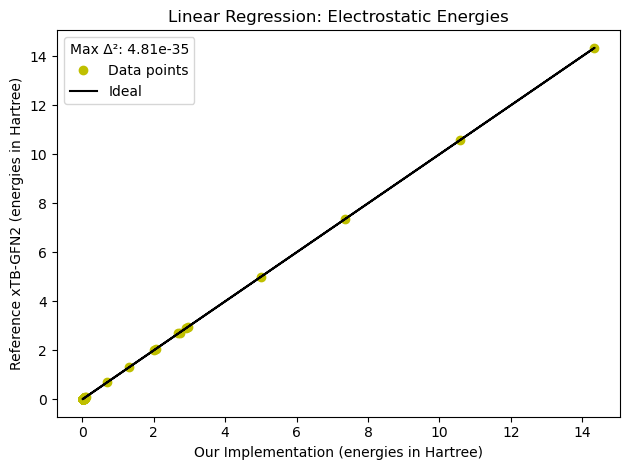
\includegraphics[width=.9\linewidth]{images/results/es_check}
  \label{fig:es_check}
\end{subfigure}%
\begin{subfigure}{.5\textwidth}
  \centering
  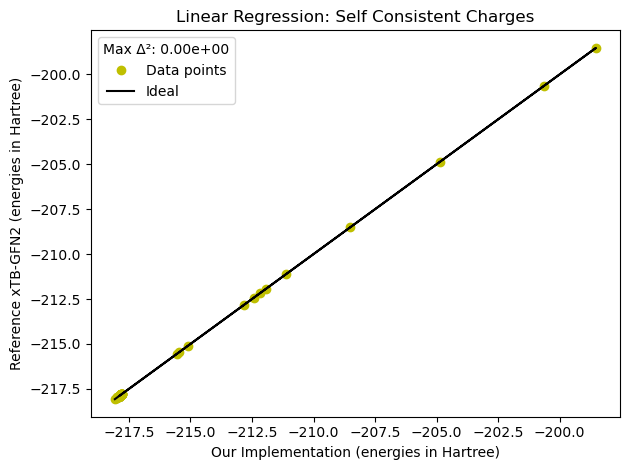
\includegraphics[width=.9\linewidth]{images/results/scc_check}
  \label{fig:scc_check}
\end{subfigure}
\caption{Linear regressions showing how much the Python implementation for the electrostatic term deviates from the Fortran results.}
\label{fig:validation_electro_precision}
\end{figure}

We can see that the results for the self-consistent charges match exactly, and that the maximum squared deviation for the electrostatic energies is miniscule. \autoref{fig:tests-output} shows the results from our comparison tests.

\begin{figure}[H]
\begin{minted}{bash}
    matches! [olapp]
    matches! [multipole_3d]
    matches! [multipole_3d_simple]
    matches! [horizontal_shift]
    matches! [form_product]
    matches! [horizontal_shift_simple]
    matches! [form_product_simple]
    matches! [dtrf2]
    li and lj are 0 for all calls, so s is not actually modified ToT
    AKA all dtrf2 calls are essentially skipped...
    matches! [get_multiints]
    [build_overlap_dipol_quadrupol] S: Is not close!
    ...
    matches! [build_overlap_dipol_quadrupol]
    matches! [build_SDQH0]
    matches! [dim_basis]
    matches! [atovlp]
    matches! [new_basis_set]
    matches! [electro]
    matches! [coordination_number]
    matches! [h0scal]
\end{minted}
\caption{Truncated output of our comparison tests.}
\label{fig:tests-output}
\end{figure}

\section{Benchmarks}
